% !TEX TS-program = lualatex
% !TEX encoding = UTF-8 Unicode
\documentclass[tikz, border=0mm, multi=page]{standalone}

% Thêm lmodern để fix toàn bộ cảnh báo thiếu size font toán học (OML/cmm)
\usepackage{lmodern}
\usepackage{fontspec}

\IfFontExistsTF{Times New Roman}{
  \setmainfont{Times New Roman}
}{
  \setmainfont{Liberation Serif}
}

\usepackage{xcolor}
\usepackage{pgfplots}
\usepackage{fontawesome5}
\pgfplotsset{compat=1.18}
\usetikzlibrary{calc, matrix, arrows.meta, shapes.geometric, positioning}

%── Định nghĩa màu sắc (Đồng bộ với slide.tex)
\definecolor{sap}{HTML}{0000FF}
\definecolor{cslate}{HTML}{64748B}
\definecolor{cbk}{HTML}{424242}
\definecolor{clightgray}{HTML}{F8F9FA}
\definecolor{cgry}{HTML}{757575}
\definecolor{cgr}{HTML}{2E7D32}
\definecolor{cbl}{HTML}{1565C0}
\definecolor{cneg}{HTML}{D32F2F}

%── Style biểu đồ (Đồng bộ với slide.tex)
\pgfplotsset{
  empty legend/.style={draw=none, fill=none},
  dashmod/.style={dashed, line width=2.5pt, mark=none},
  solproj/.style={solid,  line width=2.5pt, mark=none},
  hlchart/.style={
    clip=false,
    scale only axis=true,
    xmin=0.5, xmax=7.5, ymin=0, ymax=5.9,
    xtick={1,2,3,4,5,6,7},
    xticklabels={W1,W2,W3,{W4$^\star$},W5,W6,W7},
    x tick label style={font=\fontsize{15}{18}\selectfont, text=cgry!80!black},
    y tick label style={font=\fontsize{15}{18}\selectfont, text=cgry!80!black},
    grid=both,
    minor ytick={0,0.5,...,5.5},
    minor grid style={gray!8,  line width=0.15pt},
    major grid style={gray!18, line width=0.30pt},
    axis line style={gray!35,  line width=0.40pt},
    tick style={gray!35, line width=0.40pt},
    legend style={
      at={(0.5, -0.12)},
      anchor=north,
      font=\fontsize{14}{17}\selectfont,
      draw=none, fill=none,
      legend columns=4,
      column sep=4ex,
      row sep=1ex
    },
    legend cell align=left,
  }
}

\begin{document}

% PAGE 1: Sơ đồ gameLoop
\begin{tikzpicture}[
    box/.style={rectangle, draw=black!80, thick, text width=8cm, align=left, rounded corners=3mm, inner sep=10pt, font=\small},
    arrow/.style={-{Stealth[scale=1.5]}, line width=1.5pt, draw=gray!80},
    label/.style={font=\footnotesize\bfseries, align=center, text=black!70}
]
\node[box, fill=blue!5] (story) at (0, 4.5) {
    \textbf{\large 1. MỞ KHOÁ TUYẾN TRUYỆN}\\
    \textit{(Phân hệ cốt truyện)}\\[1ex]
    $\bullet$ \textbf{Đầu vào:} Điểm và thời gian của vòng chơi trước.\\
    $\bullet$ \textbf{Tác động:} Phân tích di sản để bẻ nhánh cốt truyện. Tạo lựa chọn mới với độ khó tương ứng.\\
    $\bullet$ \textbf{Đầu ra:} Bộ thử thách ẩn để mở nhánh mới.
};
\node[box, fill=purple!5] (console) at (5, -3) {
    \textbf{\large 2. THỬ THÁCH TUYẾN TRUYỆN}\\
    \textit{(Phân hệ bảng điều khiển)}\\[1ex]
    $\bullet$ \textbf{Đầu vào:} Bộ thử thách và thông số từ phân hệ cốt truyện.\\
    $\bullet$ \textbf{Tác động:} Cập nhật giao diện. Hiển thị chủ đề tương ứng và mục tiêu.\\
    $\bullet$ \textbf{Đầu ra:} Bộ thông số cấu hình truyền thẳng vào phân hệ lõi trò chơi.
};
\node[box, fill=green!5] (core) at (-5, -3) {
    \textbf{\large 3. VƯỢT QUA THỬ THÁCH}\\
    \textit{(Phân hệ lõi trò chơi)}\\[1ex]
    $\bullet$ \textbf{Đầu vào:} Cấu hình độ khó, tốc độ rơi, điều kiện mở khóa.\\
    $\bullet$ \textbf{Tác động:} Xử lý logic giải đố. Người chơi vượt thử thách để lấy quyền năng, đẩy cao thành tích.\\
    $\bullet$ \textbf{Đầu ra:} Kết quả thực chiến lưu lại làm dữ liệu đầu vào.
};
\draw[arrow] (story.south east) to[bend left=20] node[label, right=2mm] {Chuyển giao\\Thử thách \& Cấu hình} (console.north);
\draw[arrow] (console.west) to[bend left=15] node[label, below=2mm] {Kích hoạt\\lối chơi cốt lõi} (core.east);
\draw[arrow, draw=cneg] (core.north) to[bend left=20] node[label, left=2mm, text=cneg] {\textbf{TÁI KHỞI ĐỘNG}\\Trả kết quả thực chiến\\để định đoạt tương lai} (story.south west);
\end{tikzpicture}

% PAGE 2: Use Case gameCore
\begin{tikzpicture}
    \begin{scope}[scale=1.35, every node/.append style={transform shape}]
        \draw[cslate, thick, rounded corners=4pt] (0,0) rectangle (7.5,-5.5);
        \node[anchor=north, font=\fontsize{12}{14}\selectfont\bfseries\color{sap}] at (3.75, -0.2) {Sơ đồ usecase (chính)};
        \node (p) [circle, draw=cslate, fill=clightgray, minimum size=0.8cm] at (-1.6, -2.7) {};
        \node[below=2pt, font=\fontsize{11}{13}\selectfont\color{cbk}] at (p.south) {Người chơi};
        \node (net) [circle, draw=sap, fill=clightgray, minimum size=0.8cm] at (9.1, -2.7) {};
        \node[below=2pt, font=\fontsize{11}{13}\selectfont\color{cbk}] at (net.south) {Bộ máy Vật lý};
        \begin{scope}[every node/.style={ellipse, draw=cslate, fill=white, minimum width=3.5cm, inner sep=2pt, font=\fontsize{9}{11}\selectfont\color{cbk}}]
            \node (u1) at (3.75,-1.1) {Di chuyển \& Xoay khối};
            \node (u2) at (3.75,-2.0) {Gia tốc rơi (Drop)};
            \node (u3) at (3.75,-2.9) {Tính toán Va chạm};
            \node (u4) at (3.75,-3.8) {Xóa hàng \& Tính điểm};
            \node (u5) [draw=sap, font=\fontsize{9}{11}\selectfont\bfseries\color{sap}] at (3.75,-4.7) {Ghi nhận Thành tích};
        \end{scope}
        \foreach \i in {1,2} \draw[->, thick, draw=cslate] (p) -- (u\i.west);
        \foreach \i in {3,4,5} \draw[->, thick, draw=sap] (net) -- (u\i.east);
        \draw[->, thick, dashed, draw=sap] (u3.north) to[bend right=30] (u1.east);
    \end{scope}
\end{tikzpicture}

% PAGE 3: Use Case gameConsole
\begin{tikzpicture}
    \begin{scope}[scale=1.35, every node/.append style={transform shape}]
        \draw[cslate, thick, rounded corners=4pt] (0,0) rectangle (7.5,-5.5);
        \node[anchor=north, font=\fontsize{12}{14}\selectfont\bfseries\color{sap}] at (3.75, -0.2) {Sơ đồ usecase (Cấu hình)};
        \node (p) [circle, draw=cslate, fill=clightgray, minimum size=0.8cm] at (-1.6, -2.7) {};
        \node[below=2pt, font=\fontsize{11}{13}\selectfont\color{cbk}] at (p.south) {Người chơi};
        \node (net) [circle, draw=sap, fill=clightgray, minimum size=0.8cm] at (9.1, -2.7) {};
        \node[below=2pt, font=\fontsize{11}{13}\selectfont\color{cbk}] at (net.south) {Cloudflare D1};
        \begin{scope}[every node/.style={ellipse, draw=cslate, fill=white, minimum width=3.5cm, inner sep=2pt, font=\fontsize{9}{11}\selectfont\color{cbk}}]
            \node (u1) at (3.75,-1.1) {Tùy chỉnh hệ thống};
            \node (u2) at (3.75,-2.0) {Chọn nhánh cốt truyện};
            \node (u3) at (3.75,-2.9) {Tra cứu xếp hạng};
            \node (u4) at (3.75,-3.8) {Điều phối luồng chơi};
            \node (u5) [draw=sap, font=\fontsize{9}{11}\selectfont\bfseries\color{sap}] at (3.75,-4.7) {Đồng bộ Dữ liệu};
        \end{scope}
        \foreach \i in {1,2,3,4} \draw[->, thick, draw=cslate] (p) -- (u\i.west);
        \draw[->, thick, draw=sap] (net) -- (u5.east);
        \draw[->, thick, dashed, draw=sap] (u5.north) to[bend right=30] (u3.east);
    \end{scope}
\end{tikzpicture}

% PAGE 4: Use Case gameStory
\begin{tikzpicture}
    \begin{scope}[scale=1.35, every node/.append style={transform shape}]
        \draw[cslate, thick, rounded corners=4pt] (0,0) rectangle (7.5,-5.5);
        \node[anchor=north, font=\fontsize{12}{14}\selectfont\bfseries\color{sap}] at (3.75, -0.2) {Sơ đồ usecase (Tuyến truyện)};
        \node (p) [circle, draw=cslate, fill=clightgray, minimum size=0.8cm] at (-1.6, -2.7) {};
        \node[below=2pt, font=\fontsize{11}{13}\selectfont\color{cbk}] at (p.south) {Người chơi};
        \node (net) [circle, draw=sap, fill=clightgray, minimum size=0.8cm] at (9.1, -2.7) {};
        \node[below=2pt, font=\fontsize{11}{13}\selectfont\color{cbk}] at (net.south) {Máy chủ};
        \begin{scope}[every node/.style={ellipse, draw=cslate, fill=white, minimum width=3.5cm, inner sep=2pt, font=\fontsize{9}{11}\selectfont\color{cbk}}]
            \node (u1) at (3.75,-1.1) {Xem/Bỏ qua intro};
            \node (u2) at (3.75,-2.0) {Đọc hội thoại};
            \node (u3) at (3.75,-2.9) {Lựa chọn nhánh};
            \node (u4) at (3.75,-3.8) {Nhận thông báo};
            \node (u5) [draw=sap, font=\fontsize{9}{11}\selectfont\bfseries\color{sap}] at (3.75,-4.7) {Đồng bộ Gist API};
        \end{scope}
        \foreach \i in {1,2,3,4} \draw[->, thick, draw=cslate] (p) -- (u\i.west);
        \draw[->, thick, draw=sap] (net) -- (u5.east);
        \draw[->, thick, dashed, draw=sap] (u5.north) to[bend right=30] (u2.east);
    \end{scope}
\end{tikzpicture}

% PAGE 5: Biểu đồ trống (Bạn gọi các macro \addplot từ slide.tex nên chỉ cần khung trục)
% Lưu ý: Trong file slide.tex của bạn, bạn đã dùng lệnh \begin{axis} trực tiếp đè lên khung ảnh PDF.
% Do đó, trang 5 trong file này đóng vai trò như một base map (nếu bạn cần).
% Nếu slide.tex tự vẽ axis thì không cần trang này nữa.
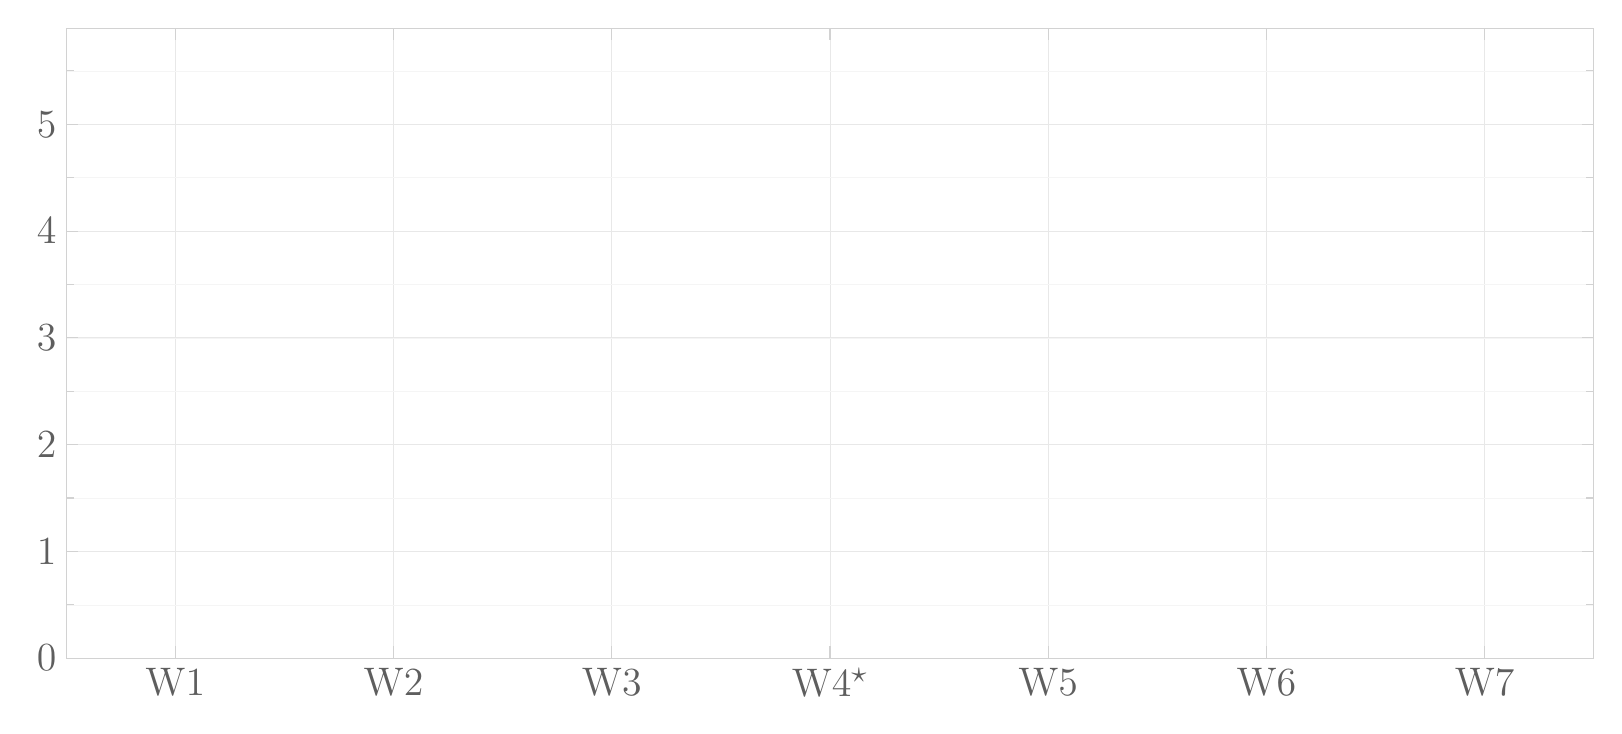
\begin{tikzpicture}
    \begin{axis}[width=194mm,height=80mm,hlchart]
        % Khung được load thẳng từ slide.tex, ta để trống data ở đây.
    \end{axis}
\end{tikzpicture}

% PAGE 6: Sơ đồ lớp và CSDL
\begin{tikzpicture}
    \begin{scope}[
        classbox/.style={rectangle, draw=cslate, line width=1.5pt, rounded corners=4pt, fill=clightgray, font=\fontsize{12}{16}\selectfont\color{cbk}, text width=55mm, align=center, inner sep=8pt},
        layerlabel/.style={font=\fontsize{16}{20}\selectfont\bfseries\color{sap}, anchor=west},
        arrow/.style={->, line width=1.5pt, draw=cslate}
    ]
        % ================= LAYER 1: gameStory =================
        \node[layerlabel] at (0, 0) {1. Phân hệ Tuyến truyện};
        \node[classbox] (story_db) at (11.5, 0) {\textbf{gameStory\_db.h}\\(SQLite \& Gist API Sync)};
        \node[classbox] (story_layout) at (19.0, 0) {\textbf{gameStory\_layout.h}\\(States \& Transitions)};
        \node[classbox] (story_assets) at (26.5, 0) {\textbf{gameStory\_assets}\\(SVG Logos \& TTF Fonts)};
        \draw[arrow] (story_db) -- (story_layout);
        \draw[arrow] (story_assets) -- (story_layout);

        \draw[cslate, dashed, line width=1pt] (0, -2) -- (29.5, -2);
        
        % ================= LAYER 2: gameConsole =================
        \node[layerlabel] at (0, -4) {2. Phân hệ Cấu hình};
        \node[classbox] (console_layout) at (11.5, -4) {\textbf{gameConsole\_layout.h}\\\texttt{SettingsConfig} Struct};
        \node[classbox] (console_db) at (19.0, -4) {\textbf{gameConsole\_db.h}\\\texttt{StoryRow} \& \texttt{Records}};
        \node[classbox] (console_sort) at (26.5, -4) {\textbf{gameConsole\_sort.h}\\Smart Sorting Engine (7 Algos)};
        \draw[<->, line width=1.5pt, draw=cslate] (console_layout) -- (console_db);
        \draw[arrow] (console_sort) -- (console_db);

        \draw[cslate, dashed, line width=1pt] (0, -6) -- (29.5, -6);
        
        % ================= LAYER 3: gameCore =================
        \node[layerlabel] at (0, -8) {3. Phân hệ Lõi trò chơi};
        \node[classbox] (core_state) at (11.5, -8) {\textbf{gameCore\_layout.h}\\\texttt{GameState} (Vòng lặp \& Cờ)};
        \node[classbox] (core_tetro) at (19.0, -8) {\textbf{Tetromino Struct}\\\texttt{blocks[4]} \& \texttt{colorID}};
        \node[classbox] (core_point) at (26.5, -8) {\textbf{Point Struct}\\\texttt{x, y} (Tọa độ ma trận)};
        \draw[arrow] (core_state) -- (core_tetro);
        \draw[arrow] (core_tetro) -- (core_point);

        \draw[cslate, dashed, line width=1pt] (0, -10) -- (29.5, -10);
        
        % ================= LAYER 4: Utilities =================
        \node[layerlabel] at (0, -12) {4. Tiện ích Hệ thống};
        \node[classbox, fill=black!8, draw=cbk] (util_logger) at (15.25, -12) {\textbf{logger.h}\\\texttt{Logger} (Singleton, \texttt{game.log})};
        \node[classbox, fill=black!8, draw=cbk] (util_debug) at (22.75, -12) {\textbf{ctetris\_debug.h}\\(HTTP Macros, WASM/Native)};
        \draw[<->, dashed, line width=1.5pt, draw=cbk] (util_logger) -- (util_debug);
    \end{scope}
\end{tikzpicture}

\end{document}